% ============================================================================
% TP Sistemas de Computación – Informe completo
% Índice: GINI + Python + C (32 bits) + Ensamblador NASM + GDB
% ============================================================================
\documentclass[a4paper,12pt]{article}
\catcode`\_=12

% ----------------------- Paquetes básicos ----------------------------------
\usepackage[utf8]{inputenc}
\usepackage[T1]{fontenc}
\usepackage[spanish]{babel}
\usepackage{graphicx}
\usepackage{subcaption}
\usepackage{caption}
\usepackage{listings}
\usepackage{amsmath}
\usepackage{float}
\usepackage{geometry}
\usepackage{fancyhdr}
\usepackage{enumitem}
\usepackage{booktabs}
\usepackage[hidelinks]{hyperref}
\usepackage{cleveref}
\usepackage{xcolor}
\usepackage{listings}

% ----------------------- Configuración global ------------------------------
\geometry{margin=2.5cm}
\graphicspath{{images/}}
\pagestyle{fancy}
\fancyhf{}
\lhead{Boot}
\rhead{TP Sistemas de Computación}
\cfoot{\thepage}

% ----------------------- Listings ------------------------------------------
\lstdefinelanguage{NASM}{
  morekeywords   ={section,global,extern,fld,fistp,add,leave,ret,push,mov,sub},
  sensitive      =true,
  morecomment    =[l]{;},
  morestring     =[b]",
}
\lstdefinelanguage{C}{
  morekeywords   ={EFI_STATUS,CHAR16,UINTN,UINT32,EFI_GUID},
  sensitive      =true,
  morecomment    =[l]{//},
  morecomment    =[s]{/*}{*/},
  morestring     =[b]",
}
\lstset{
  basicstyle   =\ttfamily\small,
  numberstyle  =\tiny,
  numbers      =left,
  stepnumber   =1,
  frame        =single,
  captionpos   =b,
  keywordstyle =\color{blue},
  commentstyle =\itshape\color{gray!70},
  language     =C      % Idioma por defecto; cambia con [language=NASM] cuando haga falta
}

% ----------------------- Metadatos del documento ---------------------------
\title{\textbf{TP Sistemas de Computación}\\\large Práctico: UEFI}
\author{Alumno: Nombre Apellido \\ Materia: Sistemas de Computación \\ Comisión: XX}
\date{\today}

% ----------------------- Inicio del documento ------------------------------
\begin{document}

\begin{titlepage}
    \begin{center}
        {\LARGE \textbf{Universidad Nacional de Córdoba}}\\[1.5cm]

        
\includegraphics[scale=0.4]{images/logo2.png}\\[1.5cm]

        {\large Facultad de Ciencias Exactas, Físicas y Naturales}\\
        {\large Escuela de Electrónica y Computacion}\\[1cm]

        \rule{\linewidth}{0.5mm}\\[0.4cm]
        {\Large \textbf{Cátedra de Sistemas de Computacion}}\\[0.3cm]
        {\LARGE \textbf{Trabajo de Laboratorio 3}}\\[0.3cm]

        \rule{\linewidth}{0.5mm}\\[1cm]

        \begin{flushleft}
        {\large 
            \textbf{Profesor Titular:} Ing. Javier Alejandro JORGE\\
            \textbf{Profesor Adjunto:} -\\[0.5cm]
            \textbf{Integrantes:}\\
            Trucchi, Genaro\\
            Trachtta, Agustin\\
            Rodriguez, Mateo\\
        }
        \end{flushleft}

        \vfill

        {\large \today}
    \end{center}
\end{titlepage}

\tableofcontents
\clearpage

\section{Introducción}

En este trabajo práctico se aborda la arquitectura UEFI, sus diferencias fundamentales
con el antiguo BIOS, la forma de interactuar con ella tanto a nivel usuario como a
nivel desarrollador, y se muestra un ejemplo de llamada a una de sus funciones de
\emph{Runtime Services}.

\section{¿Qué es UEFI?}

UEFI (\emph{Unified Extensible Firmware Interface}) es la especificación que define una
interfaz de software moderna entre el firmware de la plataforma (antes BIOS) y el
sistema operativo. A diferencia del BIOS tradicional, UEFI:
\begin{itemize}[noitemsep]
  \item Está escrito en C y opera en modo 32 o 64 bits.
  \item Ofrece controladores propios para hardware básico (red, almacenamiento, gráficos).
  \item Soporta particiones GPT (superando el límite de 2 TB de MBR).
  \item Incorpora un entorno seguro (\emph{Secure Boot}) y gestión de clave pública.
  \item Se organiza en \emph{Boot Services} (solo durante el arranque) y
        \emph{Runtime Services} (disponibles para el SO tras el \texttt{ExitBootServices}).
\end{itemize}

\subsection{¿Cómo puedo usarlo?}

\subsubsection*{Como usuario final}
\begin{enumerate}[noitemsep]
  \item Durante el arranque, pulsar la tecla indicada (DEL, F2, F10, F12, ESC) para
        entrar en el \emph{Setup} de UEFI.
  \item Desde allí se puede:
    \begin{itemize}[noitemsep]
      \item Cambiar el orden de arranque.
      \item Habilitar/deshabilitar \emph{Secure Boot}.
      \item Ajustar parámetros de hardware (incluido overclocking).
    \end{itemize}
  \item En sistemas UNIX-like, utilidades como \texttt{efibootmgr} permiten listar y
        modificar entradas UEFI desde el sistema operativo.
\end{enumerate}

\subsubsection*{Como desarrollador / cargador de arranque}
\begin{enumerate}[noitemsep]
  \item El firmware UEFI pasa al cargador una estructura \texttt{EFI\_SYSTEM\_TABLE},
        que incluye punteros a:
    \begin{itemize}[noitemsep]
      \item \texttt{BootServices} (servicios disponibles solo durante el arranque).
      \item \texttt{RuntimeServices} (servicios que perduran tras el \texttt{ExitBootServices}).
    \end{itemize}
  \item Para invocar una rutina UEFI, se localiza el puntero en la tabla de servicios
        y se llama en C/C++ correctamente, respetando la ABI UEFI
        (registro de parámetros, alineamiento, etc.).
\end{enumerate}

\newpage

\subsection{Ejemplo de llamada a función UEFI}

Una aplicación UEFI puede acceder a las variables persistentes almacenadas en la NVRAM (Non-Volatile RAM) mediante los \emph{Runtime Services}, que son parte del entorno estándar definido por la especificación UEFI. A continuación, se muestra un ejemplo de cómo utilizar la función \texttt{GetVariable} para leer la variable global \texttt{BootOrder}, la cual contiene el orden de dispositivos para el arranque del sistema. Esta función está documentada en la sección correspondiente de la especificación oficial UEFI.
\begin{lstlisting}[language=C,
                   caption={Lectura de la variable \texttt{BootOrder}},
                   label={lst:getvariable}]
#include <Uefi.h>
#include <Library/UefiLib.h>
#include <Library/UefiBootServicesTableLib.h>

extern EFI_GUID gEfiGlobalVariableGuid;

EFI_STATUS LeerBootOrder(VOID)
{
    EFI_STATUS status;
    CHAR16 *VariableName = L"BootOrder";
    UINTN DataSize = sizeof(UINT16) * 16;     // espacio para 16 entradas
    UINT16 BootOrder[16];
    UINT32 Attributes;

    status = gST->RuntimeServices->GetVariable(
        VariableName,
        &gEfiGlobalVariableGuid,
        &Attributes,
        &DataSize,
        BootOrder
    );

    if (EFI_ERROR(status)) {
        Print(L"Error al leer BootOrder: %r\n", status);
        return status;
    }
    // Procesar BootOrder...
    return EFI_SUCCESS;
}
\end{lstlisting}

\noindent Más detalles en la
\href{https://uefi.org/specs/UEFI/2.10/08_Services_Runtime_Services.html}%
      {\textcolor{blue}{especificación oficial}}.

\newpage

\section{Casos de bugs de UEFI explotables}
Los bugs en UEFI son particularmente peligrosos porque el firmware se ejecuta antes que el sistema operativo y con privilegios muy altos (equivalente a Ring $-2$ o superior, conceptualmente). Explotarlos puede llevar a ataques muy persistentes y sigilosos (bootkits). Algunos casos notables:

\begin{itemize}[noitemsep]
  \item \textbf{LoJax (2018)}: considerado el primer rootkit UEFI in the wild', usado por el grupo APT28 (Fancy Bear). Modificaba directamente la SPI flash del firmware para inyectar un módulo malicioso que persistía incluso tras reinstalar el sistema operativo o cambiar el disco duro. Aprovechaba vulnerabilidades y configuraciones inseguras que permitían escritura no autorizada en la flash de firmware.

  \item \textbf{MosaicRegressor (2020)}: framework de spyware basado en UEFI desarrollado por HackingTeam. Utilizaba imágenes de firmware comprometidas para reinstalar el malware en el sistema operativo cada vez que se eliminaba, asegurando persistencia a nivel de firmware.

  \item \textbf{ThinkPwn (2016)}: vulnerabilidad en ciertos firmwares de Lenovo (y potencialmente otros fabricantes) en la gestión de llamadas SMM (System Management Mode). Permitía a un atacante con privilegios de administrador en el SO escalar a SMM, desde donde podía modificar el firmware UEFI protegido.

  \item \textbf{LogoFAIL (2023)}: conjunto de desbordamientos de búfer en parsers de imágenes de logo personalizados usados por muchos fabricantes de UEFI durante la fase DXE (Driver Execution Environment). Un atacante podía cargar una imagen de logo maliciosa que explotara este bug, obteniendo ejecución de código arbitrario en arranque temprano.

  \item \textbf{Vulnerabilidades en drivers UEFI específicos}: de forma recurrente se descubren bugs (por ejemplo, buffer overflows) en drivers de red, USB, almacenamiento, etc. Si un atacante controla los datos procesados por estos drivers (p. ej. un USB malicioso o un paquete de red manipulado), puede desencadenar la vulnerabilidad y ejecutar código con privilegios de firmware.
\end{itemize}

\newpage

\section{Converged Security and Management Engine (CSME) e Intel Management Engine BIOS Extension (MEBx)}

\textbf{Converged Security and Management Engine (CSME) / Intel Management Engine (ME):}  
Es un subsistema de microcontrolador autónomo integrado en el chipset (Platform Controller Hub, PCH) de la mayoría de las placas base Intel desde 2006/2008. Funciona de forma independiente de la CPU y del sistema operativo, con su propio firmware (basado en MINIX), memoria y acceso directo a hardware crítico (RAM, red, periféricos). Sus principales funciones son:
\begin{itemize}[noitemsep]
  \item \emph{Intel Active Management Technology (AMT):} administración remota fuera de banda (OOB) — encender/apagar, consola remota, incluso si el SO no responde.
  \item \emph{Inicialización temprana de hardware:} parte de la configuración del sistema antes de que el BIOS/UEFI principal tome el control.
  \item \emph{Funciones de seguridad:}  
    \begin{itemize}[noitemsep]
      \item Intel Boot Guard: verifica la firma criptográfica del firmware UEFI.
      \item Intel Platform Trust Technology (PTT): implementación de TPM en firmware.
      \item Gestión de DRM (Protected Audio Video Path, PAVP), etc.
    \end{itemize}
\end{itemize}
Su naturaleza de “caja negra” propietaria con acceso privilegiado ha generado preocupaciones de seguridad; a lo largo de los años se han descubierto vulnerabilidades críticas en el ME/CSME.

\medskip
\textbf{Intel Management Engine BIOS Extension (MEBx):}  
Es el módulo de configuración integrado en el firmware principal (BIOS/UEFI) que permite ajustar las funciones del ME/AMT. Se accede normalmente al presionar \texttt{Ctrl+P} (o la combinación específica del fabricante) durante el POST. Desde MEBx se puede:
\begin{itemize}[noitemsep]
  \item Habilitar/deshabilitar AMT.
  \item Configurar parámetros de red para gestión OOB (dirección IP, VLAN, DNS).
  \item Establecer contraseñas y políticas de acceso al ME.
  \item Activar KVM remoto y otras opciones avanzadas de control.
\end{itemize}

\section{coreboot}

\textbf{¿Qué es coreboot?}  
coreboot es un proyecto de firmware libre y minimalista que reemplaza el BIOS/UEFI propietario. Su filosofía es inicializar únicamente el hardware esencial (CPU, RAM, chipset básico) y luego transferir el control a un \emph{payload} especializado.

\medskip
\textbf{Payloads comunes:}
\begin{itemize}[noitemsep]
  \item \texttt{SeaBIOS}: interfaz BIOS tradicional para compatibilidad con SOs antiguos.
  \item \texttt{TianoCore (EDK II)}: implementación de UEFI completa para SOs modernos.
  \item \texttt{GRUB2} / \texttt{U-Boot}: cargadores de arranque con gran flexibilidad.
  \item \texttt{LinuxBoot}: utiliza el kernel de Linux como payload para entornos Linux “bare-metal”.
\end{itemize}

\newpage

\medskip
\textbf{Productos que lo incorporan:}
\begin{itemize}[noitemsep]
  \item \emph{Chromebooks} de Google (firmware estándar).
  \item Laptops y desktops de fabricantes enfocados en Linux / privacidad (System76, Purism).
  \item Diversos sistemas embebidos, routers, servidores y dispositivos de red.
  \item Comunidad de porting a placas base de escritorio y portátiles de múltiples marcas.
\end{itemize}

\medskip
\textbf{Ventajas de su utilización:}
\begin{itemize}[noitemsep]
  \item \emph{Velocidad de arranque} muy superior al firmware propietario.
  \item \emph{Flexibilidad y personalización}: elección de payloads y fácil adaptación al hardware.
  \item \emph{Seguridad y transparencia}: código auditables, menor superficie de ataque (aunque a veces requiere \emph{blobs} propietarios para componentes críticos).
  \item \emph{Control total} sobre el proceso de arranque y eliminación de código heredado innecesario.
\end{itemize}

\section{Linker}

\subsection{¿Qué es un linker?}
Un linker (enlazador) es una herramienta fundamental en el proceso de desarrollo de software. Actúa como un “ensamblador” de piezas de código y datos provenientes de diferentes fuentes para crear un único archivo de salida.

\subsection{¿Qué hace?}
Sus tareas principales son:

\begin{itemize}[noitemsep]
  \item \textbf{Combinación de secciones de código y datos:} Los archivos objeto (\texttt{.o}) generados por el ensamblador o el compilador contienen secciones como \texttt{.text} (código), \texttt{.data} (datos inicializados) y \texttt{.bss} (datos no inicializados). El linker toma todas las secciones homónimas de los distintos archivos y las une en una sola sección en el archivo de salida, siguiendo un script de linker (\texttt{link.ld}) o las reglas por defecto.
  
  \item \textbf{Resolución de símbolos:} Cuando el código referencia símbolos (por ejemplo, el nombre de una función como \texttt{\_start} o una etiqueta de datos como \texttt{msg}), el linker busca su definición entre todos los archivos objeto y bibliotecas de entrada. Luego sustituye cada uso simbólico por la dirección final donde ese símbolo ha sido colocado en el archivo de salida. Si falta una definición, se produce un error de “referencia no definida”; si hay definiciones duplicadas, un error de “definición múltiple”.

  \item \textbf{Relocalización:} Los archivos objeto contienen direcciones provisionales o relativas. El linker ajusta (o “parchea”) estas direcciones para que apunten a las ubicaciones finales en el ejecutable resultante, teniendo en cuenta la dirección base especificada en el script del linker (por ejemplo, \texttt{0x7C00} en un bootloader). Esto incluye tanto saltos internos como referencias a símbolos externos.

  \item \textbf{Generación del archivo de salida:} Finalmente, escribe el resultado combinado, resuelto y relocalizado en un archivo. El formato puede ser un ejecutable estándar del sistema operativo (ELF, PE) o, si se solicita explícitamente (con \texttt{--oformat binary}), una imagen binaria cruda sin cabeceras adicionales.
\end{itemize}

\section{¿Qué es la dirección 0x7C00 y por qué es necesaria?}

La dirección \texttt{0x7C00} es un estándar histórico en la arquitectura x86 que corresponde al punto de memoria física donde el BIOS carga el primer sector arrancable (MBR o VBR, 512 bytes) de un dispositivo seleccionado para el arranque. Su importancia y necesidad en el script del linker se sustenta en varios aspectos:

\begin{itemize}[noitemsep]
  \item \textbf{Convención del BIOS:} Cuando una PC compatible arranca en modo legado (BIOS o UEFI CSM), el firmware busca un dispositivo arrancable, lee su primer sector (512 bytes) y lo copia en la dirección física \texttt{0x7C00}. Inmediatamente después, establece los registros \texttt{CS:IP} a \texttt{0000:7C00} y salta a esa dirección para comenzar la ejecución.

  \item \textbf{Cálculo de direcciones finales:} El código ensamblado (\texttt{main.S}) incluye referencias a sus propias etiquetas (por ejemplo, la dirección de la cadena \texttt{msg} o el destino del salto \texttt{jmp print\_loop}). Para que esas referencias apunten a las ubicaciones correctas durante la ejecución (cuando el código resida en \texttt{0x7C00}), el linker *debe* conocer esta dirección base durante el proceso de enlace. Al indicar \texttt{. = 0x7C00} al principio de la sección \texttt{SECTIONS} en el script \texttt{link.ld}, le decimos al linker: “Considera que el inicio del código estará en \texttt{0x7C00} y calcula todas las direcciones relativas a esta base”.

  \item \textbf{Relocalización adecuada:} Gracias a esa directiva (\texttt{. = 0x7C00}), el linker puede calcular la dirección absoluta correcta para cada símbolo y referencia interna. Por ejemplo, si la etiqueta \texttt{msg} está a un desplazamiento de 26 bytes desde el inicio (\texttt{\_start}), el linker codificará su dirección como \texttt{0x7C00 + 26 = 0x7C1A} dentro de la instrucción \texttt{movw \$msg, \%si}.

  \item \textbf{Evitar desajustes catastróficos:} Si el linker no supiera la dirección de carga \texttt{0x7C00} (por ejemplo, si asumiera una base 0), calcularía todas las direcciones internas de forma incorrecta respecto al punto de carga real. Cuando el BIOS cargase el código en \texttt{0x7C00}, una instrucción como \texttt{movw \$msg, \%si} cargaría una dirección errónea (ej., 0x1A en lugar de 0x7C1A). El programa fallaría inmediatamente al intentar leer la cadena o realizar saltos, probablemente causando un cuelgue o reinicio.
\end{itemize}

\newpage % Inicia la sección práctica en una nueva página

\section{Demostración Práctica: Compilación, Enlace y Depuración}

Para ilustrar los conceptos anteriores, se realizó el proceso completo para crear, verificar y depurar un pequeño programa "Hello World" que funciona como un sector de arranque MBR en modo real de 16 bits.

\subsection{Compilación con el Ensamblador (as)}

El primer paso es convertir el código fuente en ensamblador (\texttt{main.S}, que contiene la directiva \texttt{.code16} para indicar que es código de 16 bits) en un archivo objeto (\texttt{main.o}).

\begin{lstlisting}[style=BashInputStyle, caption=Comando de ensamblaje inicial]
as -o main.o main.S
\end{lstlisting}

Sin embargo, al ejecutar esto en un sistema operativo host de 64 bits (como Ubuntu x86\_64), el ensamblador \texttt{as}, aunque genera las instrucciones correctas de 16 bits gracias a \texttt{.code16}, crea un archivo objeto ELF que internamente está marcado con la arquitectura \texttt{x86-64}. Esto causa conflictos posteriores con el linker cuando se intenta generar una salida \texttt{i386}.

Para mitigar esto, se puede intentar forzar a \texttt{as} a usar un formato más tradicional o directamente usar una Máquina Virtual Linux de 32 bits o un compilador cruzado (\textit{cross-compiler}) \texttt{i686-elf-as}. Una opción que a veces funciona es:
\begin{lstlisting}[style=BashInputStyle, caption=Intento de comando de ensamblaje (puede variar)]
as --traditional-format -o main.o main.S
\end{lstlisting}
(Nota: La solución más fiable para evitar estos problemas es usar una VM de 32 bits o un compilador cruzado.)

\subsection{Enlace con el Linker (ld)}

Una vez obtenido el archivo objeto \texttt{main.o}, se utiliza el linker \texttt{ld} junto con el script \texttt{link.ld} para generar la imagen binaria final \texttt{main.img}.

\begin{lstlisting}[style=BashInputStyle, caption=Comando de enlace]
ld -m elf_i386 -T link.ld -o main.img main.o
\end{lstlisting}

Explicación de las opciones:
\begin{itemize}[noitemsep]
    \item \texttt{-m elf\_i386}: Esencial para resolver conflictos de arquitectura. Indica a \texttt{ld} que procese la entrada y genere (internamente antes de convertir a binario) para la arquitectura \texttt{i386}. Asegura la compatibilidad con el objetivo y \texttt{OUTPUT\_ARCH(i386)} del script.
    \item \texttt{-T link.ld}: Especifica que se deben usar las reglas definidas en el archivo \texttt{link.ld}. Este script establece la dirección base en \texttt{0x7C00}, organiza las secciones \texttt{.text}, \texttt{.data}, etc., y asegura (mediante \texttt{.org}/\texttt{.word} en \texttt{main.S} o directivas del linker) que la imagen final tenga 512 bytes y la firma MBR \texttt{0xAA55} en los últimos dos bytes.
    \item \texttt{-o main.img}: Nombre del archivo de salida.
    \item \texttt{main.o}: Archivo objeto de entrada.
\end{itemize}
El resultado es el archivo \texttt{main.img}, una imagen binaria cruda de 512 bytes lista para ser arrancada.

\subsection{Verificación (objdump vs. hd)}

Para visualizar el trabajo de relocalización realizado por el linker, comparamos la salida del desensamblador sobre el archivo objeto con un volcado hexadecimal de la imagen binaria final.

\begin{lstlisting}[style=BashInputStyle, caption=Comandos de verificación]
objdump -d main.o
hd main.img 
# o hexdump -C main.img
\end{lstlisting}

Qué comparar:
\begin{itemize}[noitemsep]
    \item \textbf{Desensamblado (\texttt{objdump}):} Muestra las instrucciones máquina y sus direcciones relativas (usualmente desde 0) dentro del archivo objeto. Por ejemplo, para \texttt{movw \$msg, \%si}, muestra la instrucción y una dirección \textit{relativa} para \texttt{msg} (ej., \texttt{0x1a}). Los bytes hexadecimales codificarán esta dirección relativa (ej., \texttt{be 1a 00}).
    \item \textbf{Volcado Hexadecimal (\texttt{hd}):} Muestra los bytes crudos del archivo \texttt{main.img}. Al buscar la misma secuencia de bytes para \texttt{movw \$msg, \%si} (empezará con \texttt{be}), se observa que los bytes de la dirección \textit{han cambiado}. En lugar de \texttt{1a 00}, ahora se verá la dirección \textit{absoluta} calculada por el linker usando \texttt{0x7C00} como base (ej., \texttt{1a 7c}, correspondiente a \texttt{0x7C1A} en little-endian). Esta diferencia demuestra la relocalización.
    \item \textbf{Firma MBR:} En la salida de \texttt{hd}, se verifica que los dos últimos bytes del archivo (offsets \texttt{0x1fe} y \texttt{0x1ff}) son \texttt{55 aa}.
\end{itemize}

\subsection{Depuración con QEMU y GDB}

Finalmente, se depura la ejecución del MBR usando el emulador QEMU y el depurador GDB.

\subsubsection{Iniciar QEMU en modo depuración}

\begin{lstlisting}[style=BashInputStyle, caption=Lanzar QEMU esperando a GDB]
qemu-system-i386 -fda main.img -boot a -s -S
\end{lstlisting}
Explicación de las opciones:
\begin{itemize}[noitemsep]
    \item \texttt{-fda main.img}: Carga \texttt{main.img} como disquete A. (Ajustar ruta si es necesario).
    \item \texttt{-boot a}: Indica a QEMU arrancar desde el disquete A.
    \item \texttt{-s}: Inicia un servidor GDB en \texttt{localhost:1234}.
    \item \texttt{-S}: Congela la CPU al inicio, esperando que GDB se conecte y dé la orden de continuar.
\end{itemize}
QEMU se inicia pero queda pausado.

\subsubsection{Sesión de GDB}

Se abre otra terminal y se inicia GDB.

\begin{enumerate}[noitemsep]
    \item \textbf{Conectar a QEMU:}
        \begin{lstlisting}[style=GdbStyle]
(gdb) target remote localhost:1234 
        \end{lstlisting}
        Se establece la conexión. GDB muestra la dirección inicial (\texttt{0x0000fff0}) y una advertencia sobre la falta de un ejecutable especificado, lo cual es normal.
    
    \item \textbf{Cargar Símbolos (Opcional pero recomendado):} Para usar etiquetas del código fuente.
        \begin{lstlisting}[style=GdbStyle]
(gdb) file main.o
        \end{lstlisting}
        GDB podría mostrar una advertencia sobre incompatibilidad de arquitecturas entre el archivo \texttt{.o} (marcado como x86-64 por \texttt{as}) y el objetivo \texttt{i386} reportado por QEMU. Sin embargo, en la práctica, a menudo GDB logra cargar los símbolos de todas formas.


    \item \textbf{Establecer Arquitectura (¡CRUCIAL!):} Indicar a GDB que interprete el código como 16 bits.
        \begin{lstlisting}[style=GdbStyle]
(gdb) set architecture i8086
        \end{lstlisting}
        
    \item \textbf{Establecer Breakpoint Inicial:} Detener la ejecución al inicio de nuestro código MBR.
        \begin{lstlisting}[style=GdbStyle]
(gdb) b *0x7c00
        \end{lstlisting}
        
    \item \textbf{Iniciar Ejecución:} Decirle a GDB que deje correr a QEMU.
        \begin{lstlisting}[style=GdbStyle]
(gdb) c
Continuing.
        \end{lstlisting}
        QEMU simula el final del BIOS, carga \texttt{main.img} y salta a \texttt{0x7c00}, donde GDB detiene la ejecución debido al breakpoint.
        \begin{figure}[H]
            \centering
            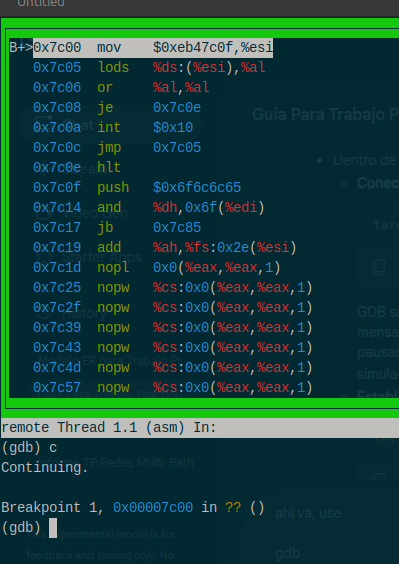
\includegraphics[width=0.8\textwidth]{images/break7C00.png}
            \caption{GDB detenido en el breakpoint en 0x7c00. Layout `asm` muestra el código.}
        \end{figure}

    \item \textbf{Ejecutar Paso a Paso y Observar:} Se utiliza \texttt{si} (Step Instruction) para avanzar instrucción por instrucción.
        \begin{itemize}
            \item Con \texttt{info registers} (o \texttt{layout regs}), se observa el cambio en los registros \texttt{ax}, \texttt{ds}, \texttt{es} (inicialización a 0) y \texttt{si} (carga de la dirección de \texttt{msg}).
              \begin{figure}[H]
                  \centering
                  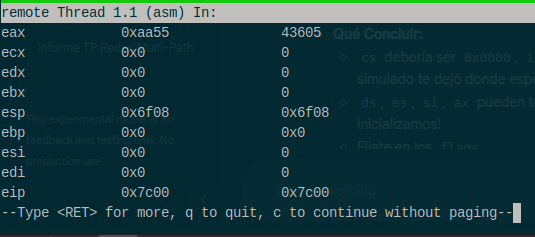
\includegraphics[width=0.8\textwidth]{images/registers7c00.png}
                  \caption{Salida parcial de `info registers` al inicio.}
              \end{figure}
            \item Se sigue el bucle \texttt{print\_loop}:
              \begin{figure}[H]
                  \centering
                  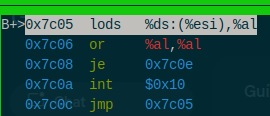
\includegraphics[width=0.6\textwidth]{images/bucle.png}
                  \caption{Instrucciones del bucle de impresión en GDB.}
              \end{figure}
              Se observa cómo \texttt{lods} carga un carácter en \texttt{al} e incrementa \texttt{si}. 
              Esa imagen representa el bucle donde se carga letra por letra el 'hello world'
        \end{itemize}

    \item \textbf{Correr hasta el Final:} Para ver el resultado completo:
        \begin{lstlisting}[style=GdbStyle]
(gdb) b halt # Poner breakpoint en la etiqueta halt
(gdb) c      # Continuar hasta halt
        \end{lstlisting}
        Se observa el mensaje completo en QEMU. GDB se detiene en la instrucción \texttt{cli} en \texttt{halt}.

    \item \textbf{Últimas Instrucciones:} Con \texttt{si}, se ejecuta \texttt{cli} (se verifica el flag \texttt{IF} desactivado con \texttt{info registers flags}) y luego \texttt{hlt}. Al ejecutar \texttt{hlt}, la CPU simulada se detiene. GDB ya no puede avanzar más. Se sale de GDB con \texttt{quit}.
    \begin{figure}[H]
        \centering
        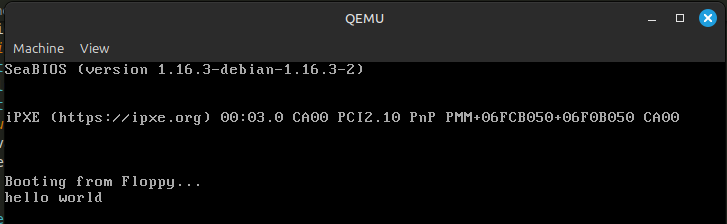
\includegraphics[width=0.8\textwidth]{images/resultado.png}
        \caption{Resultado final.}
    \end{figure}
\end{enumerate}

\end{document}
\section{Creación y prueba de un bootloader básico}

\subsection{Objetivo}

El objetivo de esta práctica es comprender el proceso de creación de un \textbf{bootloader} sencillo, capaz de ejecutarse directamente al arrancar una computadora, sin la intervención de un sistema operativo.

\subsection{Conceptos fundamentales}

Un bootloader es el primer fragmento de código ejecutado por el procesador luego del encendido. Cuando la BIOS finaliza sus rutinas de inicialización, busca un sector de arranque (\textit{boot sector}) en los dispositivos conectados. Este sector debe cumplir las siguientes condiciones:
\begin{itemize}
    \item Tener un tamaño de \textbf{512 bytes}.
    \item Terminar con la \textbf{firma mágica} \texttt{0xAA55}.
    \item El código debe asumir que será cargado en la dirección de memoria física \textbf{0x7C00}.
\end{itemize}

\subsection{Procedimiento realizado}

\subsubsection{Creación del código en ensamblador}

Se escribió un programa en lenguaje ensamblador NASM que imprime caracteres en pantalla utilizando servicios de la BIOS:

\begin{lstlisting}[language={[x86masm]Assembler}, caption={Código del bootloader básico}]
[org 0x7C00]

mov ah, 0x0E
mov al, 'H'
int 0x10

mov al, 'E'
int 0x10

mov al, 'L'
int 0x10

mov al, 'L'
int 0x10

mov al, 'O'
int 0x10

hlt

times 510-($-$$) db 0
dw 0xAA55
\end{lstlisting}

\textbf{Explicación}:
\begin{itemize}
    \item \texttt{[org 0x7C00]}: indica que el código debe pensar que se ejecuta a partir de la dirección \texttt{0x7C00}.
    \item \texttt{mov ah, 0x0E} + \texttt{int 0x10}: llama a una interrupción BIOS para imprimir un carácter en pantalla en modo texto.
    \item \texttt{times 510-(\$-\$\$) db 0}: rellena con ceros hasta llegar a 510 bytes.
    \item \texttt{dw 0xAA55}: agrega la firma mágica necesaria para que la BIOS reconozca el sector como booteable.
\end{itemize}

\subsubsection{Compilación}

Se utilizó NASM para ensamblar el código directamente a un archivo binario plano:

\begin{lstlisting}[language=bash, caption={Compilación del bootloader}]
nasm -f bin main.asm -o main.img
\end{lstlisting}

\subsubsection{Prueba en máquina virtual}

Antes de grabarlo en hardware real, se utilizó \textbf{QEMU} para probar el funcionamiento de la imagen:

\begin{lstlisting}[language=bash, caption={Ejecución en QEMU}]
qemu-system-x86_64 -drive format=raw,file=main.img -display sdl
\end{lstlisting}

Esto lanzó una ventana de emulación donde se pudo observar la impresión de ``HELLO'' en la pantalla al arrancar.

\subsubsection{Opcional: grabación en un pendrive físico}

Para probar el bootloader en hardware real, se puede grabar el archivo en un pendrive siguiendo precauciones extremas para no sobrescribir otros dispositivos:

\begin{lstlisting}[language=bash, caption={Grabación en dispositivo USB}]
sudo dd if=main.img of=/dev/sdX bs=512 count=1 status=progress
\end{lstlisting}

donde \texttt{sdX} debe ser reemplazado por el identificador correcto del pendrive.

\subsection{Resultados}

Se logró exitosamente ejecutar un programa de arranque que imprime texto en pantalla, tanto en entorno virtualizado como en condiciones aptas para hardware real.

\begin{figure}[H]
    \centering
    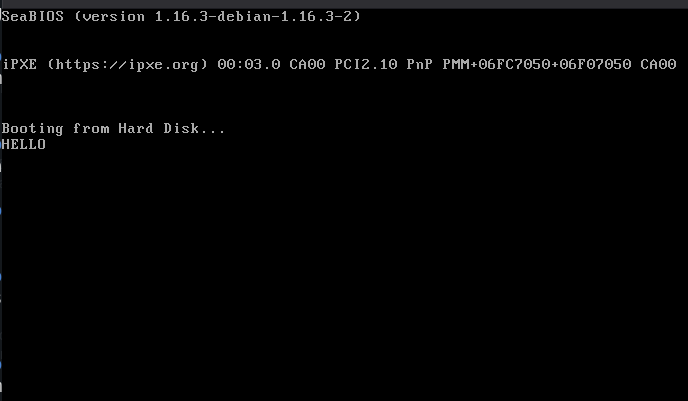
\includegraphics[width=0.5\textwidth]{images/bootloader_hello.png}
    \caption{Bootloader mostrando ``HELLO'' en QEMU.}
\end{figure}

\subsection{Conclusiones}

\subsubsection{Prueba en hardware real}

Una vez comprobado el funcionamiento del bootloader en entorno virtualizado, se procedió a grabarlo en un dispositivo USB físico y probarlo en una computadora real.

Los pasos realizados fueron:

\begin{enumerate}
    \item Conectar únicamente el pendrive para evitar confusiones con otros discos.
    \item Identificar el dispositivo correcto mediante el comando:
    \begin{lstlisting}[language=bash]
lsblk
    \end{lstlisting}
    \item Desmontar la partición montada del pendrive:
    \begin{lstlisting}[language=bash]
sudo umount /dev/sdc1
    \end{lstlisting}
    \item Grabar la imagen del bootloader en el dispositivo completo:
    \begin{lstlisting}[language=bash]
sudo dd if=main.img of=/dev/sdc bs=512 count=1 status=progress
    \end{lstlisting}
    \item Expulsar de forma segura el pendrive:
    \begin{lstlisting}[language=bash]
sudo eject /dev/sdc
    \end{lstlisting}
    \item Insertar el pendrive en la computadora de prueba, acceder al \textit{Boot Menu} durante el arranque (presionando F12, F10, ESC o la tecla correspondiente) y seleccionar el pendrive como dispositivo de arranque \textbf{en modo Legacy (no UEFI)}.
\end{enumerate}

Al bootear desde el pendrive, el sistema ejecutó correctamente el bootloader, mostrando el texto programado.

\begin{figure}[H]
    \centering
    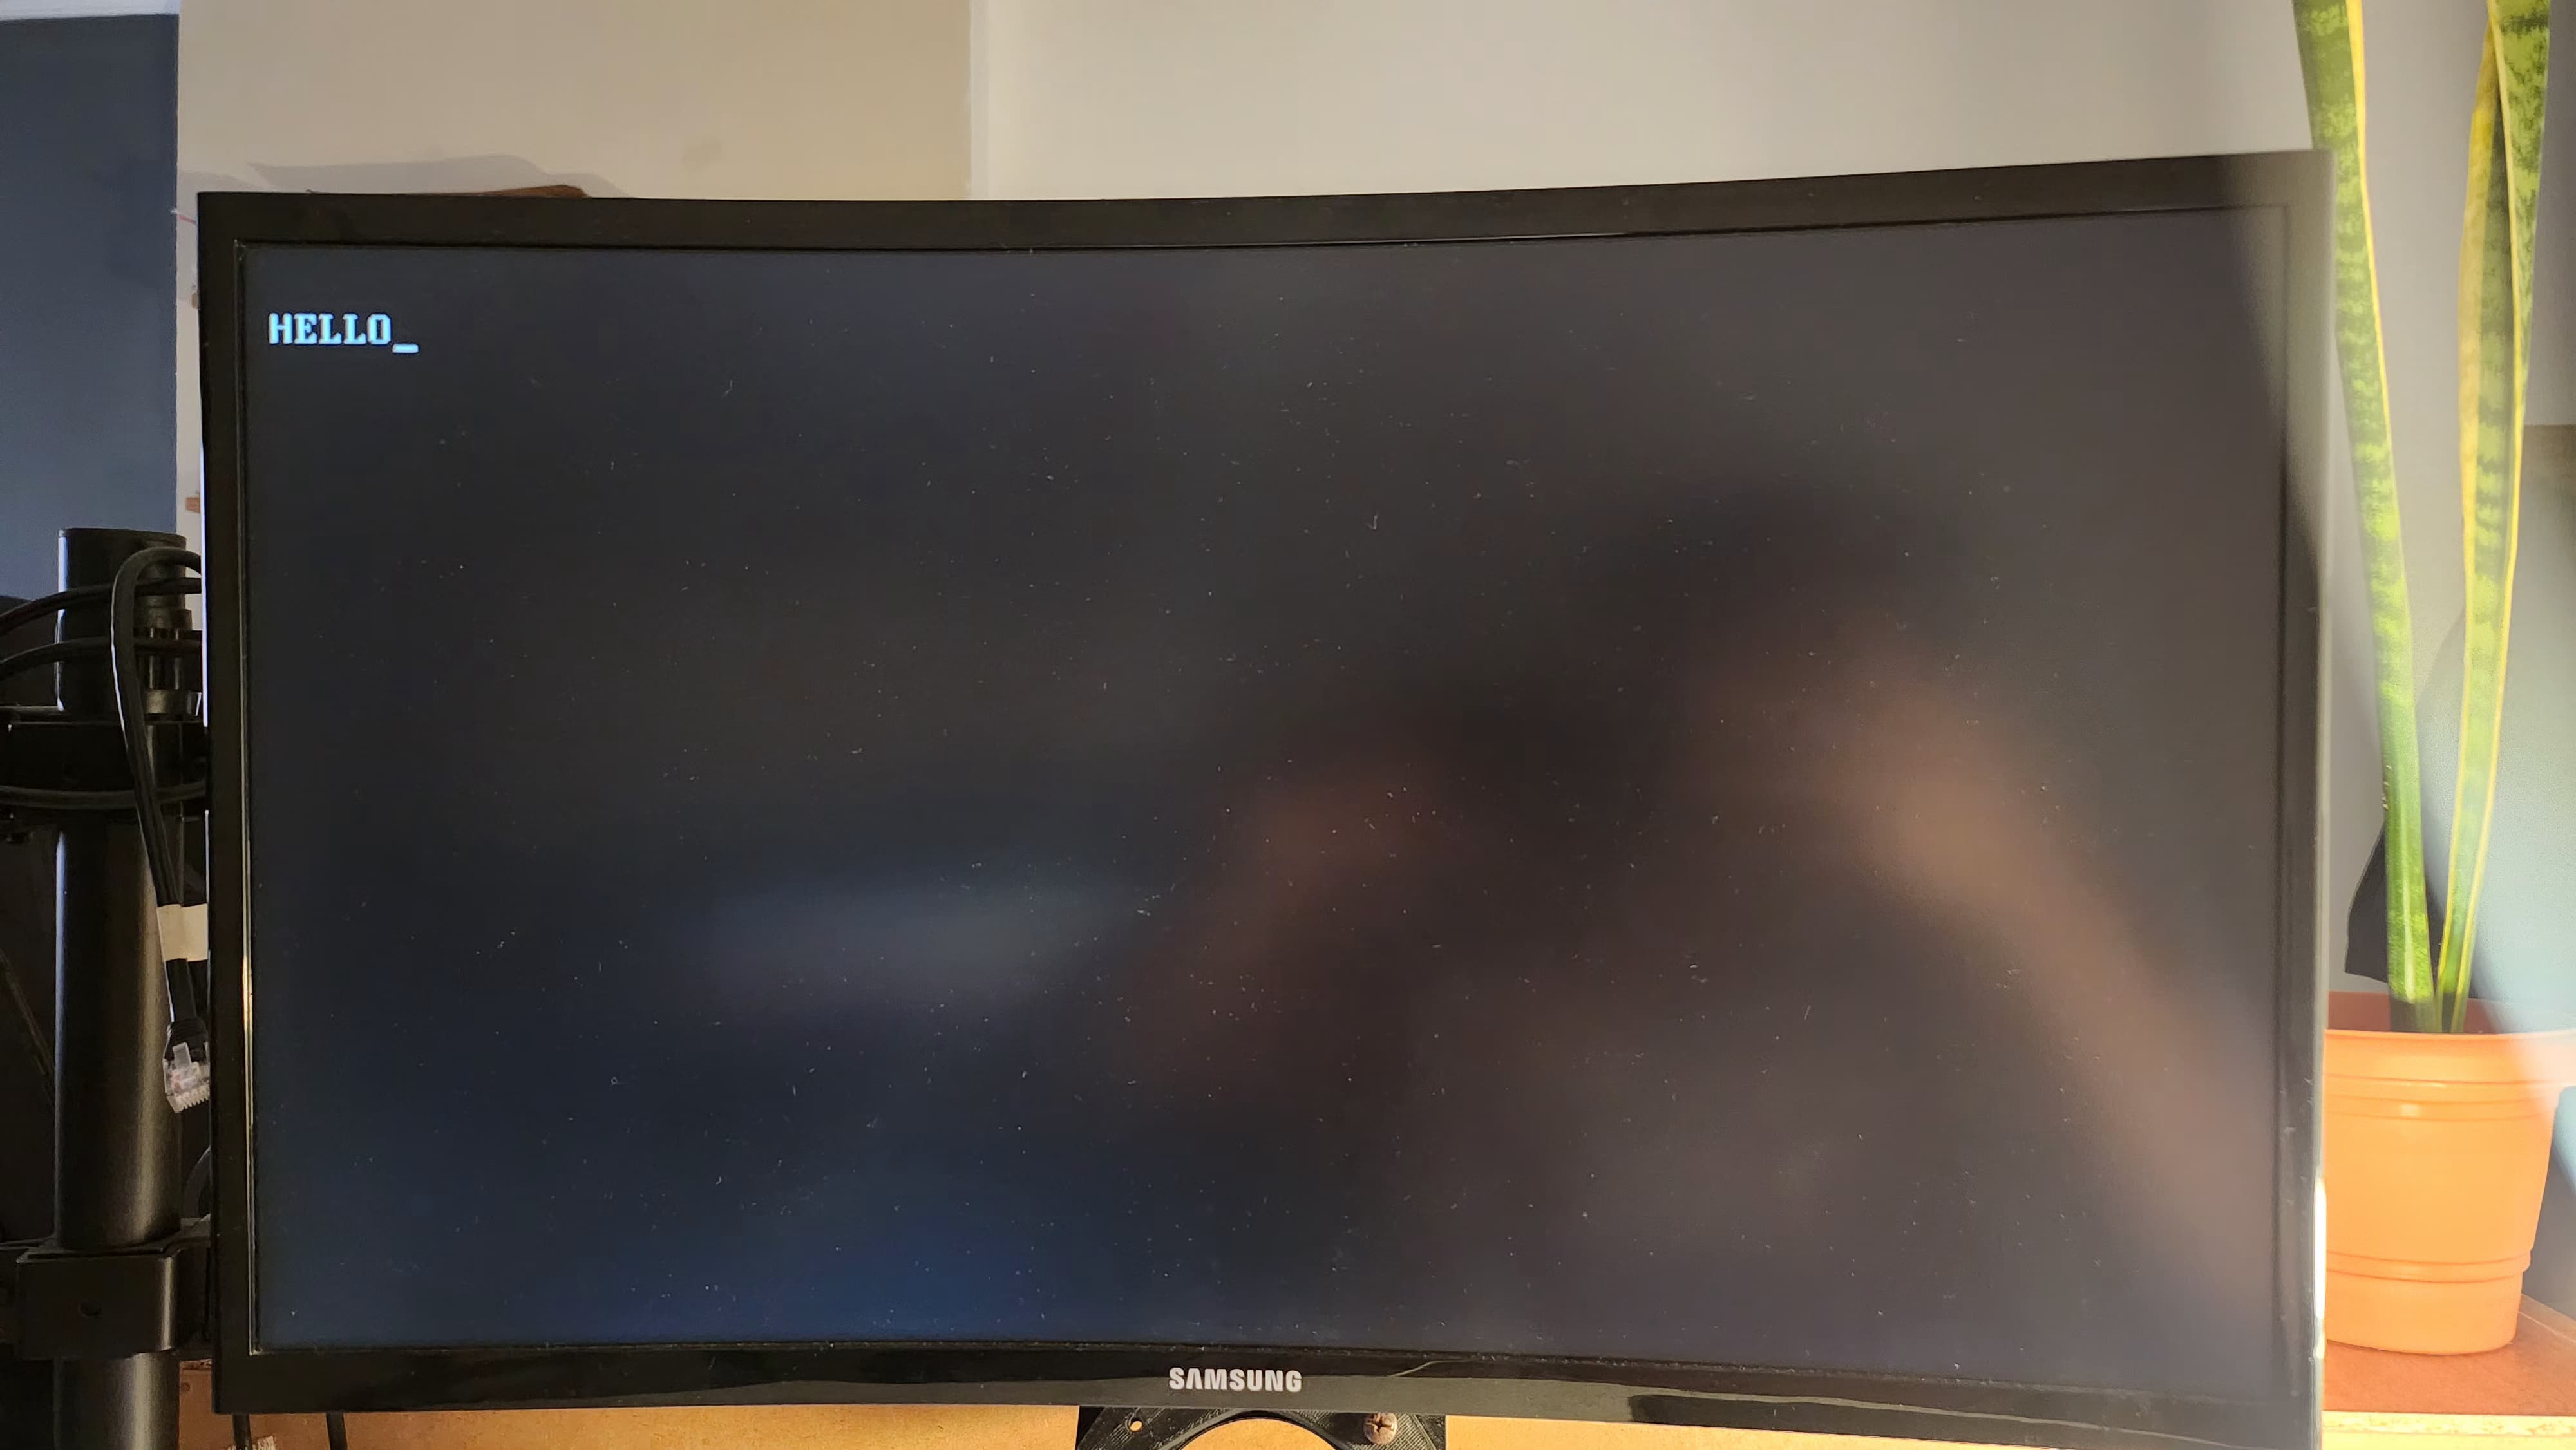
\includegraphics[width=0.5\textwidth]{images/bootloader_pendrive.jpeg}
    \caption{Bootloader mostrando ``HELLO'' desde pendrive en hardware real.}
\end{figure}

Esta práctica permitió:
\begin{itemize}
    \item Comprender el flujo de arranque de una PC desde nivel BIOS.
    \item Aplicar conocimientos de lenguaje ensamblador en un entorno de bajo nivel.
    \item Experimentar con herramientas de emulación de hardware.
\end{itemize}

Se consolidó así el conocimiento sobre cómo interactuar directamente con el hardware sin sistemas operativos intermedios.

\section{Conclusiones}

El presente trabajo práctico permitió recorrer desde los conceptos teóricos de la arquitectura \textbf{UEFI} hasta la implementación y prueba de un \emph{bootloader} propio, revelando la interacción detallada entre firmware, herramientas de \emph{toolchain} y hardware.

\begin{itemize}
  \item \textbf{UEFI como reemplazo de BIOS}. Comprendimos que UEFI no es una simple evolución sino una plataforma firmware escrita en~C, capaz de operar en 32~/ 64~bits, con servicios de arranque y ejecución en tiempo de \emph{runtime}, soporte GPT, \emph{Secure Boot} y controladores integrados. Aprender a invocar sus tablas (\texttt{BootServices} y \texttt{RuntimeServices}) habilita el desarrollo de utilidades de muy bajo nivel que conviven con el sistema operativo.
  \item \textbf{Superficie de ataque y riesgos}. Casos como \emph{LoJax}, \emph{ThinkPwn} o \emph{LogoFAIL} evidencian que vulnerar el firmware permite \emph{bootkits} persistentes aun tras reinstalar el SO. La seguridad del arranque exige tanto configuraciones correctas (protección de la flash) como la aplicación oportuna de parches.
  \item \textbf{CSME / ME y MEBx}. Las funciones de gestión remota (AMT) y arranque verificado (Boot Guard) ofrecen ventajas, pero el motor autónomo de Intel sigue siendo una \emph{caja negra} con fallos críticos publicados. Conocer MEBx resulta clave para equilibrar administración y exposición al riesgo.
  \item \textbf{coreboot: firmware libre}. coreboot demuestra que es posible reemplazar firmware propietario por una solución mínima y auditada, con arranques más veloces y menor superficie de ataque, manteniendo la flexibilidad gracias a los \emph{payloads} (SeaBIOS, TianoCore, LinuxBoot, etc.).
  \item \textbf{Herramientas de \emph{toolchain}}. Revisar el \texttt{linker} y la convención histórica de 0x7C00 mostró que los scripts de enlace son tan cruciales como el código; si el \emph{linker} desconoce la dirección final, los desplazamientos fallan y el arranque se aborta.
  \item \textbf{Bootloader ``HELLO''}. Desde ensamblar 512~bytes y firmarlos con \texttt{0xAA55}, hasta probar en QEMU y grabar en un pendrive, cerramos el ciclo completo: escribir, enlazar, testear y ejecutar código que arranca sin sistema operativo.
\end{itemize}

Además, el desafío final permitió poner en práctica conceptos clave de la transición al Modo Protegido:

\begin{itemize}
  \item \textbf{Transición Manual a Modo Protegido.} El diseño de un bootloader completamente manual, sin macros ni abstracciones, obligó a comprender en profundidad el flujo de activación del PE (Protection Enable), la importancia del salto largo posterior (\texttt{ljmp}), y la configuración explícita de los registros de segmento y la pila en 32 bits.
  \item \textbf{Uso Correcto de ELF y Linker Scripts.} La necesidad de ensamblar primero a ELF y luego enlazar usando un \texttt{link.ld} a 0x7C00 destacó el rol crítico del linker en sistemas bare-metal, resolviendo problemas típicos de formatos binarios directos (\texttt{-f bin}) como desincronizaciones y referencias incorrectas.
  \item \textbf{Segmentación y Protección.} Implementar descriptores diferenciados de código, datos R/W y datos R/O permitió experimentar directamente con la protección por hardware: definir un segmento de sólo lectura y verificar mediante ejecución que la CPU detecta y bloquea accesos inválidos.
  \item \textbf{Verificación de Protección por Hardware.} El intento de escribir en un segmento R/O, seguido de la observación de excepciones de Protección General (GP) y triple fallo en emuladores precisos como Bochs y QEMU-KVM, demostró empíricamente cómo el hardware asegura el cumplimiento de permisos segmentados, incluso antes de introducir mecanismos de paginación.
\end{itemize}

Estos ejercicios finales consolidaron no sólo la teoría del modelo de segmentación x86 y del proceso de arranque, sino también la práctica detallada de debugging en entornos reales (GDB, QEMU, Bochs), el entendimiento del rol de los selectores en modo protegido y la importancia de diseñar firmwares mínimos pero seguros.


\end{document}
